\begin{abstract}
Forkable sandboxes make it inexpensive to execute many isolated workers, but isolation does not determine how their noisy outputs should be combined. We present an \emph{uncertainty-aware reduction contract}: a worker returns an estimate, per-observation information, sample size, and provenance fields rather than an unexplained scalar. For disjoint evidence about a common parameter, established confidence-distribution pooling combines the resulting Gaussian natural parameters. Under local asymptotic normality this factor can be written as a Gibbs measure $\exp\{-\beta E(\theta)\}$ with $\beta=n$ when energy is defined per observation. The thermodynamic form is an interpretation, not a new estimator; its useful content is total precision $nJ$, an associative merge, and an exact product normalizer whose disagreement term exposes worker conflict. A public artifact validates the Gaussian algebra, the normalizer, schema and overlap checks, an unequal-size IID logistic sanity check, and a scale-aware multivariate outlier heuristic. One four-shard run restores workers from a named islo snapshot and executes the pipeline end to end. Separate Daytona and Tensorlake measurements cover default sandbox creation, not snapshot restore. We state the boundary explicitly: multiplying factors assumes independent, non-overlapping evidence and a common target; the included outlier heuristic is not a Byzantine guarantee; and forked AI agents may be correlated and miscalibrated. We therefore frame lineage- and evidence-aware reduction as the systems research agenda opened by this interface. Artifact: \url{https://github.com/zozo123/boltzmann-mapreduce}.
\end{abstract}

\section{Introduction}
\label{sec:intro}

MapReduce succeeded because a small user-defined interface let a runtime absorb partitioning, placement, retries, and communication~\cite{dean2004mapreduce}. Its reduce function is general: it can merge sufficient statistics, model parameters, or arbitrary values. The present problem is therefore not that MapReduce is restricted to arithmetic. It is that many parallel evaluation and agent pipelines still expose a scalar result while discarding how that result was produced, how uncertain it is, and whether it shares evidence with another worker.

Forkable sandboxes sharpen this problem. A warm environment can be snapshotted and restored into isolated children, making parallel tests, sampled evaluations, hyperparameter trials, and agent branches operationally convenient~\cite{agache2020firecracker,ustiugov2021reap,morph2024}. Yet a fork is an execution primitive, not an independence guarantee. Children can share model weights, prompts, repository state, tests, and an execution ancestor. Treating their outputs as independent votes can manufacture confidence from repeated versions of the same error.

We ask a narrower systems question: \emph{what result type should a forked worker return so that a reducer can combine evidence without pretending that every output is equally informative?} Our answer is a \texttt{statistical\_result} carrying an estimate $\hat\theta_k$, per-observation information $J_k$, sample size $n_k$, execution metadata, evidence identifiers, and fork lineage. The artifact rejects literal evidence-ID reuse by default and preserves lineage; modeling residual correlation among related branches remains future work.

The statistical merge is established confidence-distribution and inverse-information pooling~\cite{singh2005combining,tang2020distributed,zhou2017raocd}. Under local asymptotic normality (LAN), a worker's quadratic confidence factor has the Gibbs form $\exp\{-\beta_k E_k(\theta)\}$ under the convention $\beta_k=n_k$. Calling the integral of the product a partition function gives a compact thermodynamic reading, but does not change the estimator. We use that reading to specify the interface, derive the exact Gaussian normalizer, separate concentration from robustness, and identify what must be added for forked agents.

\noindent\textbf{Contributions.}
\begin{itemize}
  \item \textbf{Contract.} An uncertainty- and provenance-carrying worker result with an associative Gaussian canonical summary $(P,q,c,N)$, where $P=nJ$, $q=P\hat\theta$, and $c=\hat\theta^TP\hat\theta$.
  \item \textbf{Interpretation and boundary.} A thermodynamic reading of established confidence-distribution pooling, including the exact disagreement contribution to the product normalizer and explicit assumptions on independence, common targets, dimension, and local asymptotics.
  \item \textbf{Auditable artifact.} A deterministic reference implementation with validation, an associative hierarchical merge API, duplicate-evidence rejection, an exact normalizer, local statistical sanity checks, one named-snapshot islo execution, and carefully separated sandbox-creation observations on two other clouds.
  \item \textbf{Research agenda.} Lineage-aware reduction for correlated agent branches, evidence-derived rather than self-reported confidence, and robust multivariate fusion under untrusted precision.
\end{itemize}

\section{Result Contract and Execution}
\label{sec:model}

\paragraph{Worker result.} Worker $k$ emits
\begin{equation}
r_k=(\hat\theta_k,J_k,n_k,\mathcal L_k,\mathcal E_k,m_k),
\label{eq:contract}
\end{equation}
where $\mathcal L_k$ is fork lineage, $\mathcal E_k$ identifies underlying evidence, and $m_k$ records execution metadata. The reference JSON schema serializes these fields. At ingestion it rejects non-finite estimates, non-positive sample sizes, malformed provenance, inconsistent dimensions, and non-symmetric or non-positive-definite information matrices; merge rejects overlap among non-empty evidence IDs unless explicitly overridden. These checks establish structural validity and literal deduplication, not statistical independence or honesty.

For a $p$-dimensional Gaussian factor, define
\begin{equation}
P_k=n_kJ_k,\quad q_k=P_k\hat\theta_k,\quad
c_k=\hat\theta_k^TP_k\hat\theta_k.
\label{eq:canonical}
\end{equation}
Independent summaries merge by componentwise addition:
\begin{equation}
(P,q,c,N)=\bigoplus_k(P_k,q_k,c_k,n_k).
\label{eq:merge}
\end{equation}
This operation is associative and commutative, so it can be reduced hierarchically. In more than one dimension there is generally no single scalar worker weight; information is directional. The artifact reports scalar weights only for $p=1$.

\paragraph{When not to use it.} Model-specific sufficient statistics are preferable when available. A mean is recovered exactly from $(\sum_i x_i,n)$, and ordinary least squares from $(X^TX,X^Ty)$. Our contract targets one-shot settings where workers expose estimates and uncertainty but raw data or exact sufficient statistics are unavailable, undesirable to transmit, or model-specific. It does not replace exact aggregation.

\paragraph{Execution is orthogonal to inference.} The same contract can run over processes, containers, microVMs, or remote clients. The local backend uses Python's platform-dependent process pool and makes no copy-on-write claim. The islo backend builds one environment, saves a named snapshot, and restores one sandbox per shard. A committed four-shard run exercises that path. Daytona and Tensorlake scripts instead measure default sandbox create/run/delete operations; they do not restore the named islo snapshot and are not presented as equivalent restore measurements.

Forking improves environment reuse and isolation, not statistical independence. Before multiplying two factors, a production reducer must inspect $\mathcal E_k$ and $\mathcal L_k$ for shared data, shared evaluation, or branch ancestry. The artifact blocks literal evidence-ID overlap, but deliberately refuses to treat distinct IDs or distinct sandboxes as proof of independence.

\section{Statistical Foundation}
\label{sec:boltzmann}

\paragraph{Prior work and scope.} Confidence distributions combine frequentist evidence from independent sources~\cite{singh2005combining,xie2013confidence}. Rao-type confidence-distribution (Rao-CD) methods place estimating-function inference directly in a MapReduce setting~\cite{zhou2017raocd}; related work gives distributed simultaneous inference for generalized linear models~\cite{tang2020distributed}. Our Gaussian merge is this established estimator.

We assume: (i) disjoint, statistically independent evidence; (ii) a common parameter $\theta_0$ across workers; (iii) fixed $p$; (iv) positive-definite, consistently estimated information; and (v) local sample sizes large enough for LAN. Let $I_k$ denote limiting per-observation information and $J_k\overset{p}{\to}I_k$. For worker $k$,
\begin{equation}
n_k^{1/2}(\hat\theta_k-\theta_0)
\overset{d}{\longrightarrow}N(0,I_k^{-1}),
\label{eq:lan}
\end{equation}
and the leading quadratic confidence factor is
\begin{equation}
g_k(\theta)=\exp\!\left\{-\tfrac12
(\theta-\hat\theta_k)^TP_k(\theta-\hat\theta_k)\right\}.
\label{eq:factor}
\end{equation}
This factor is exact for an exactly quadratic Gaussian model with the relevant covariance treated as known. A linear estimating equation alone is insufficient for finite-sample Gaussian exactness; plug-in nuisance estimates and non-Gaussian errors generally return us to asymptotics.

\paragraph{Product mode and normalizer.} Let $P=\sum_kP_k$, $q=\sum_kq_k$, and $c=\sum_kc_k$. Completing the square gives
\begin{equation}
\hat\theta=P^{-1}q,\qquad \mathrm{Cov}(\hat\theta)=P^{-1}.
\label{eq:pool}
\end{equation}
For the unnormalized factors in Eq.~\eqref{eq:factor}, the exact integral is
\begin{equation}
Z_g=(2\pi)^{p/2}|P|^{-1/2}\exp(-\Delta/2),
\quad \Delta=c-q^TP^{-1}q\ge0.
\label{eq:normalizer}
\end{equation}
$\Delta/2$ is the minimum summed energy: it is zero when worker modes agree and increases as they conflict. The reference implementation exposes this \texttt{disagreement\_energy} and computes $-\log Z_g$ exactly. The scalar $Z_g$ itself changes with the parameterization's integration measure; under a common nonsingular linear reparameterization, $\Delta$ is invariant while $Z_g$ acquires the expected Jacobian. Normalizers should therefore be compared only under the same model and coordinates. If each local factor is normalized, its Gaussian normalization constants must additionally be included.

\paragraph{Thermodynamic convention.} Writing
\begin{equation}
E_k(\theta)=\tfrac12(\theta-\hat\theta_k)^TJ_k(\theta-\hat\theta_k),
\quad \beta_k=n_k,
\label{eq:gibbs}
\end{equation}
gives $g_k=\exp\{-\beta_kE_k\}$. This separation is conventional: $n_k$ could be absorbed into $J_k$. The invariant statistical quantity is total precision $P_k=n_kJ_k$, not sample size alone. Thus ``hot'' and ``cold'' are useful shorthand only after fixing the per-observation energy convention. If $K$ grows while each $n_k$ remains fixed, local temperatures do not fall even though total precision can increase; one may instead define a global $\beta=N=\sum_kn_k$ and a weighted average energy.

\paragraph{Concentration is not robustness.} The pooled mode depends on worker $o$ through
\begin{equation}
\frac{\partial\hat\theta}{\partial\hat\theta_o}=P^{-1}P_o.
\label{eq:influence}
\end{equation}
Low precision limits leverage, but the influence does not decay with distance: Gaussian precision pooling is unbounded in location, and false high precision adds a second attack surface. There is no ``Boltzmann suppression'' guarantee for an outlying mode.

The artifact includes a transparent stress-test heuristic: precision volume is capped using median/MAD statistics on $p^{-1}\log|P_k|$, while multivariate locations receive a redescending weight after coordinate-wise median/MAD scaling. It catches attacks outside the first coordinate and is scale-aware, but it is not rotation invariant and has no Byzantine breakdown guarantee. We retain it as a failure demonstration, not a security result.

\section{Artifact Sanity Checks and Execution Observations}
\label{sec:eval}

All statistical inputs below are synthetic. ``Real'' refers only to execution on an allocated cloud sandbox. The experiments are deterministic sanity checks, not a comprehensive efficiency or coverage study.

\begin{table}[t]
\centering\footnotesize
\caption{Committed statistical sanity checks. Gaps are distances to the centralized estimator on the same synthetic data, not estimates of repeated-sampling efficiency.}
\label{tab:stats}
\begin{tabularx}{\columnwidth}{@{}>{\raggedright\arraybackslash}p{0.25\columnwidth}>{\raggedleft\arraybackslash}X>{\raggedleft\arraybackslash}p{0.34\columnwidth}@{}}
\toprule
Scenario & Info. pool & Centralized / baseline \\
\midrule
Mean, 12 shards & $4.9542$ & mean $4.9546$ \\
Linear regression & gap $0.033$ & centralized OLS \\
Logistic, 8 seeds & gap $0.0083\pm0.0042$ & equal avg. $0.177\pm0.090$ \\
Scalar stress test & $4.9566$ after heuristic & attacked $17.0004$ \\
\bottomrule
\end{tabularx}
\end{table}

\paragraph{Gaussian algebra.} Twelve homoscedastic mean shards have sizes $107$--$355$. The information pool is $4.9542$ with a Gaussian interval $[4.8980,5.0104]$, while the full sample mean is $4.9546$. The reducer matches closed-form inverse-variance pooling to machine precision. This is an algebraic test; $(\sum x,n)$ would recover the sample mean exactly. The same implementation produces a $0.033$ coefficient gap to centralized OLS, for which $(X^TX,X^Ty)$ is again an exact alternative.

\paragraph{Unequal-size IID logistic shards.} Five shards of sizes $\{60,120,400,2000,5000\}$ share the same covariate and outcome mechanism. Across eight committed seeds, information pooling is $0.0083\pm0.0042$ from the centralized MLE; equal coefficient averaging is $0.177\pm0.090$ away. This checks the expected direction under severe size imbalance. It does not establish an advantage over sample-size weighting, Rao-CD, surrogate likelihood, or distributed Newton, and it is not a non-IID experiment.

\begin{figure}[t]
\centering
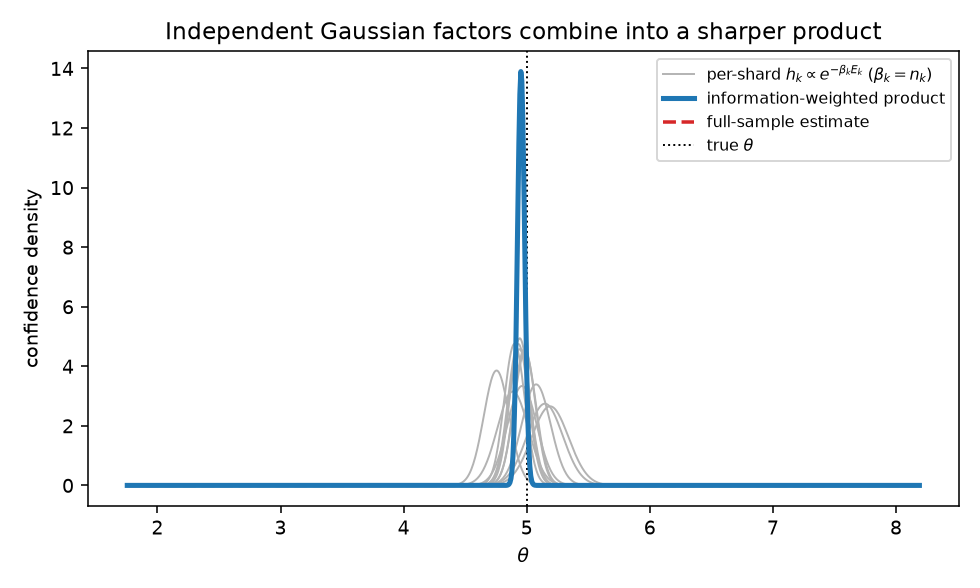
\includegraphics[width=\columnwidth]{figs/fig_gibbs.png}
\caption{Synthetic one-dimensional Gaussian factors under the per-observation energy convention. Their product is sharper; its mode lies close to the centralized sample estimate. This is a visualization of established precision pooling, not evidence of a new estimator.}
\label{fig:gibbs}
\end{figure}

\paragraph{Outlier stress test.} One synthetic scalar worker reports a far location, fabricated sample size, and $50\times$ inflated precision. Unprotected pooling moves to $17.0004$; the heuristic flags and strongly downweights the worker, returning $4.9566$. The test demonstrates both the vulnerability and one narrow mitigation. It does not support claims about collusion, adaptive attacks, high-dimensional robustness, or a Byzantine fraction.

\paragraph{Named-snapshot execution.} In one islo trial, a $141$\,MB locked parent environment was saved as a named snapshot and restored into four sandboxes. The workers returned a pooled synthetic mean $4.9422$ versus full-sample $4.9450$. Four concurrent restore-run-capture round trips completed in $6.70$\,s. Because the computation is seed-pinned, this is an execution-path existence proof rather than a statistical comparison of backends; it does not isolate in-host restore latency.

\begin{table}[t]
\centering\footnotesize
\caption{Platform-specific batched observations. Operations and timing boundaries differ, so rows are not a latency ranking. Success counts are batched totals, not simultaneous fanout.}
\label{tab:fanout}
\begin{tabularx}{\columnwidth}{@{}l>{\raggedright\arraybackslash}Xl>{\raggedright\arraybackslash}X@{}}
\toprule
Platform & Operation & Success & Reported $p_{50}$ \\
\midrule
Daytona & default create & $1024/1024$ & $0.20$\,s create \\
Tensorlake & default create & $256/256$ & $3.44$\,s create \\
islo & named restore+run & $255/256$ & $6.87$\,s round trip \\
\bottomrule
\end{tabularx}
\end{table}

\paragraph{Batched platform observations.} Under account concurrency caps, separate scripts completed 1024 Daytona default creates, 256 Tensorlake default creates, and 255 of 256 islo named-snapshot restore/run operations. These observations establish API reachability and bounded-throughput batches only. They do not compare identical images, working sets, or timing boundaries, and they do not demonstrate 256--1024 concurrent sandboxes.

\section{Failure Boundaries and Agenda}
\label{sec:agenda}

\paragraph{Dependence and double counting.} Multiplication is invalid when factors reuse observations or share correlated noise. Forked agents are especially problematic: identical model weights, prompts, tests, tools, and ancestors create common-mode errors. The implementation rejects literal evidence-ID reuse; lineage should parameterize or bound residual correlation. A useful next reducer would operate on a fork DAG and combine factors conditionally rather than treating leaves as IID.

\paragraph{Different local truths.} The common-$\theta_0$ assumption makes this a fixed-effect reducer. Under site-specific truths, $P^{-1}$ ignores between-worker variation and can be severely overconfident. Random-effects or hierarchical confidence distributions are required before claiming robustness to genuine non-IID data.

\paragraph{Agent confidence.} A model's verbal confidence is not a calibrated standard error. For agent workloads, $J_k$ should be derived from external evidence: repeated tests, held-out evaluations, independent verifiers, or empirically calibrated outcome models. Adaptive branch selection further introduces winner's-curse bias; the reducer must know which evidence was used to select survivors.

\paragraph{Systems evaluation.} The artifact does not establish a snapshot advantage over processes, containers, or cold microVMs. A full systems evaluation must run an identical workload and image across backends; measure concurrent fanout, warm-hit rate, page faults, memory sharing, p50/p95/p99 latency, failures, cost, and statistical utility per unit time; and exercise retry, idempotence, and hierarchical reduction under failure.

These limitations suggest the more consequential primitive: a fork should emit not only an answer and nominal confidence, but also evidence and dependency structure. Uncertainty-aware reduction becomes trustworthy only when the runtime can answer \emph{why} two workers should count as separate evidence.

\section{Conclusion}
\label{sec:conclusion}

We presented a result contract and an auditable reference implementation for uncertainty-aware reduction over forkable workers. The statistical merge is established confidence-distribution pooling; the thermodynamic notation is a useful convention that exposes total precision, concentration, and an exact disagreement term, not a new estimator or a robustness proof. The artifact computes that normalizer correctly, exposes an associative hierarchical merge, rejects literal duplicate evidence IDs, validates worker summaries, preserves lineage, and scopes cloud observations to the operations actually measured. The open research problem is harder and more relevant to AI systems: combining correlated, adaptively selected, and potentially miscalibrated agent evidence without double counting or trusting false precision. Forkable sandboxes make ensembles easy to execute; lineage-aware evidence reduction is what could make them scientifically useful.
